\documentclass{article}
\usepackage[utf8]{inputenc}
\usepackage[russian]{babel}
\usepackage{graphicx}
\usepackage{amsmath}
\usepackage{breqn}
\usepackage{wrapfig}
\usepackage{float}
\usepackage{multirow}
\usepackage{caption}
\usepackage{subcaption}

\graphicspath{ {./data/images} }
\author{Александр Романов Б01-107}
\title {3.4.5 Петля гистерезиса(динамический метод)}
\date{}

\begin{document}
\maketitle
\section{Введение}
\subsection{Цель работы}
Изучение петель гистерезиса различных ферромагнитных материалов в переменных полях.
\subsection{В работе используются}
Автотрансформатор, реостат, интегрирующая ячейка, амперметор, вольтметр, резистор, делитель напряжения, электронный
осциллограф, тороидальные образцы с двумя обмотками.

\section{Работа}
Запишем  некоторые характеристики образцов:
\begin{table}[H]
\centering
    \begin{tabular}{|c|c|c|c|}
        \hline
                    &Кремнистое железо  &Феррит &Пермаллой\\\hline
        $N_0$         &20                 &42     &15     \\\hline
        $N_u$         &200                &400    &300    \\\hline
        $S$, cm^2     &2                  &3      &0.66   \\\hline
        $2\pi R$, cm  &11                 &25     &14.1   \\\hline
    \end{tabular}
\end{table}
Запишем некоторые параметры установки:
\begin{table}[H]
    \centering
        \begin{tabular}{|c|c|}
            \hline
            $R_0,\; \Omega$&0.2\\\hline
            $R_u,\; k\Omega$&20\\\hline
            $C_u,\; \mu F$  &20\\\hline
        \end{tabular}
    \end{table}

\subsection{Калибровка канала X ЭО}

Закоротим обмотку \(N_0\). Ток будет синусоидален. Амперметр А подключим на измерение эффективного тока \(I_{act}\),
текущий через \(R_0\). Сигнал с этого сопротивления подадим на вход X ЭО. В этом случае ширина горизонтальной
развёртки на экране ЭО соответствует удвоеной амплитуде напряжения на \(R_0\). Измерив длину \(2x = 7\; cells\)
горизонтальной прямой на экране, ток \(I_{act} = 2.37\; A\) вычислим \(K_X\) - чувствительность канала X.

\[ K_X = \frac{2R_0\sqrt{2}I_{act}}{2x} = 0.19\; V/cell\]

\subsection{Калибровка канала Y ЭО}

Сигнал с обмотки $12.6\; V$ понижающего трансформатора подадим на делитель напряжения. Часть этого напряжения снимем
с делителя с коэффициентом 1:10 и подадим  на вход Y ЭО. Вольтметр V в это время измеряет напряжение \(U_{act}\) на
этих клеймах делителя. Измерив величину \(2y = 2\; cells\) и \(U_{act}\), расчитаем чувствительность \(K_Y\) канала Y.

\[ K_Y = \frac{2\sqrt{2}U_{act}}{2y} = 0.038\; V/cell \]

\subsection {Проверка параметров low-pass фильтра}
Проверим применимость нашей RC-цепочки. Для этого с обмотки \(6.3\; V\) поададим на неё синусоидальное напряжение
с частотой \( \nu = \omega/2\pi = 50\; Hz\)
Измерив \( U_{in} \) и \( U_{out} \) можно расчитать постоянную времени
\[ \tau = RC = U_{in}/(2\pi \nu U_{out})  = \frac{4.26\: V}{2\pi\cdot 50\: Hz \cdot 0.033\:V} = 0.41\; s\]
Также можно вычислить \(\tau\) через параметры установки \(C_u\) и \(R_u\):
\[ \tau = C_u\cdot R_u = 0.4\; s\]
Результаты совпадают. Также проверим соотношение:
\[ R_u \gg \frac{1}{\omega C_u} \]
\[ 20\cdot 10^3 \gg 159 \]
Т.е. интегрирующая ячейка прекрасно подходит для наших измерений.
\subsection{Работа}
\subsubsection{Кремнистое железо}
В ходе изучения петли гисерезиса для кремнистого железа была получено изображение:
\begin{figure}[H]
    \centering
    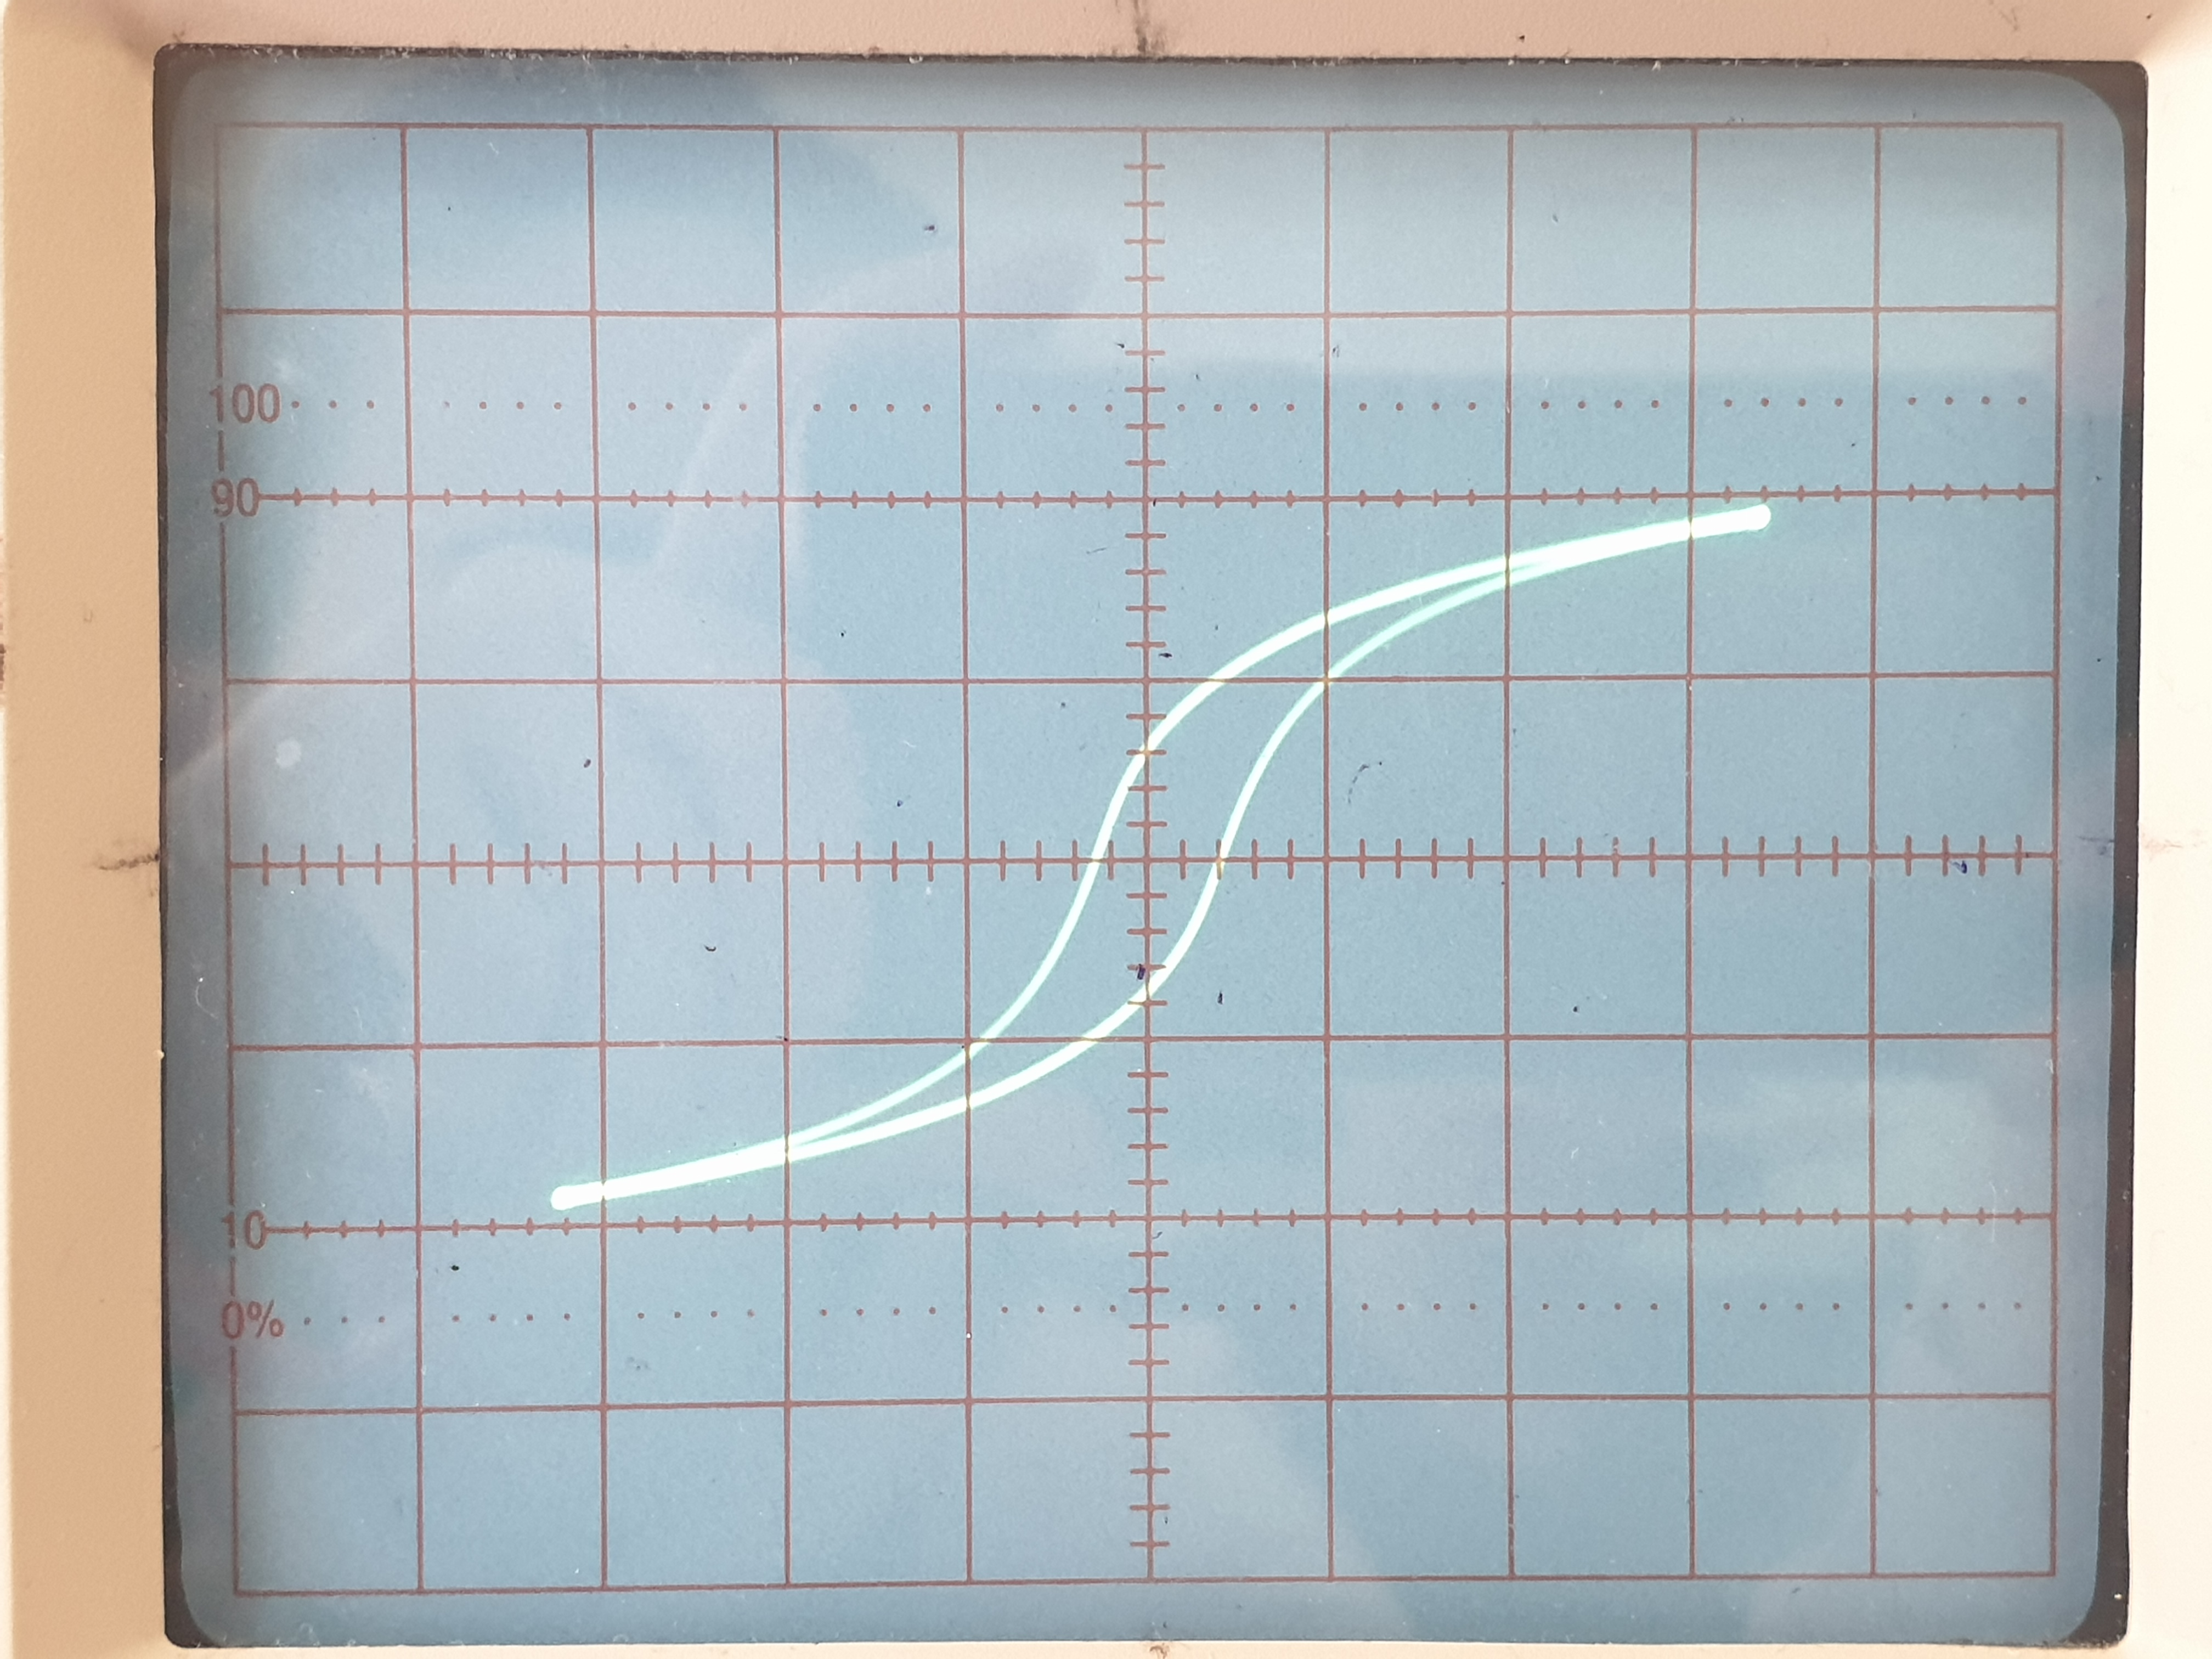
\includegraphics[width = 0.8\textwidth]{1-1.jpg}
    \caption{Петля гистерезиса для кремнистого железа}
\end{figure}

Измерения будем проводить с чувствительностями:
\[ K_X = 0.19\; V/cell,\; K_Y = 0.038\; V/cell  \]

Расчитаем цену деления наряжённости поля $H$ и индукции $B$:
\[ H = \frac{IN_0}{2\pi R} = 172.7\; A/(m\cdot cell) \]
\[ B = \frac{R_uC_u}{SN_u}U_{out} = 0.38\; T/cell \]
Теперь расчитаем коэрцетивную силу $H_c$ и индукцию насыщения $B_s$ для кремнистого железа:
\[ H_c = 120\; A/m \]
\[ B_s = 0.133\; T \]

Изменяя ток $I_{act}$ получим кривую насыщения:
\begin{figure}[H]
    \centering
    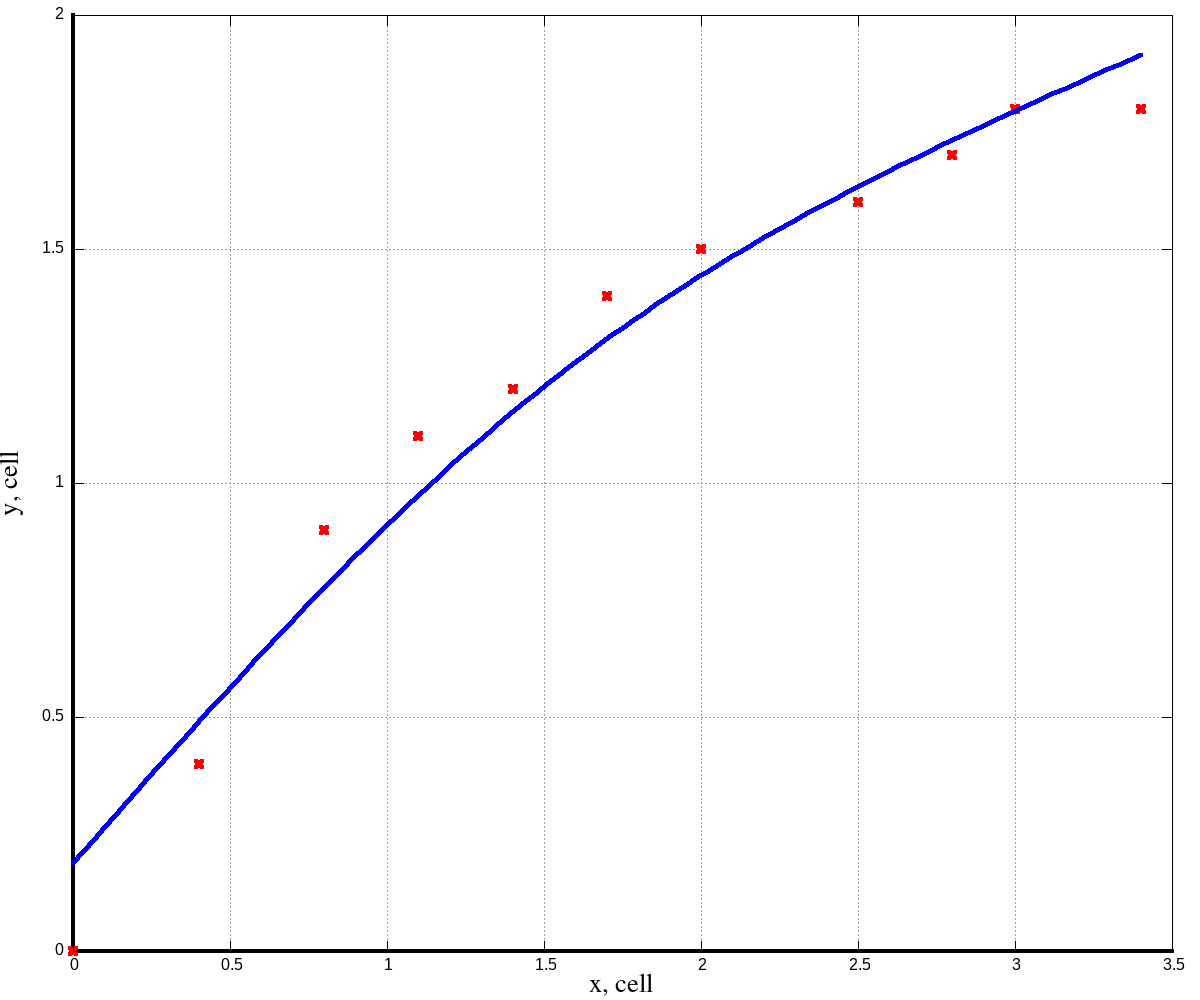
\includegraphics[width = 0.8\textwidth]{1-d.png}
    \caption{Кривая насыщения для кремнистого железа}
\end{figure}

\subsubsection{Пермаллой}
В ходе изучения петли гисерезиса для пермаллоя была получено изображение:
\begin{figure}[H]
    \centering
    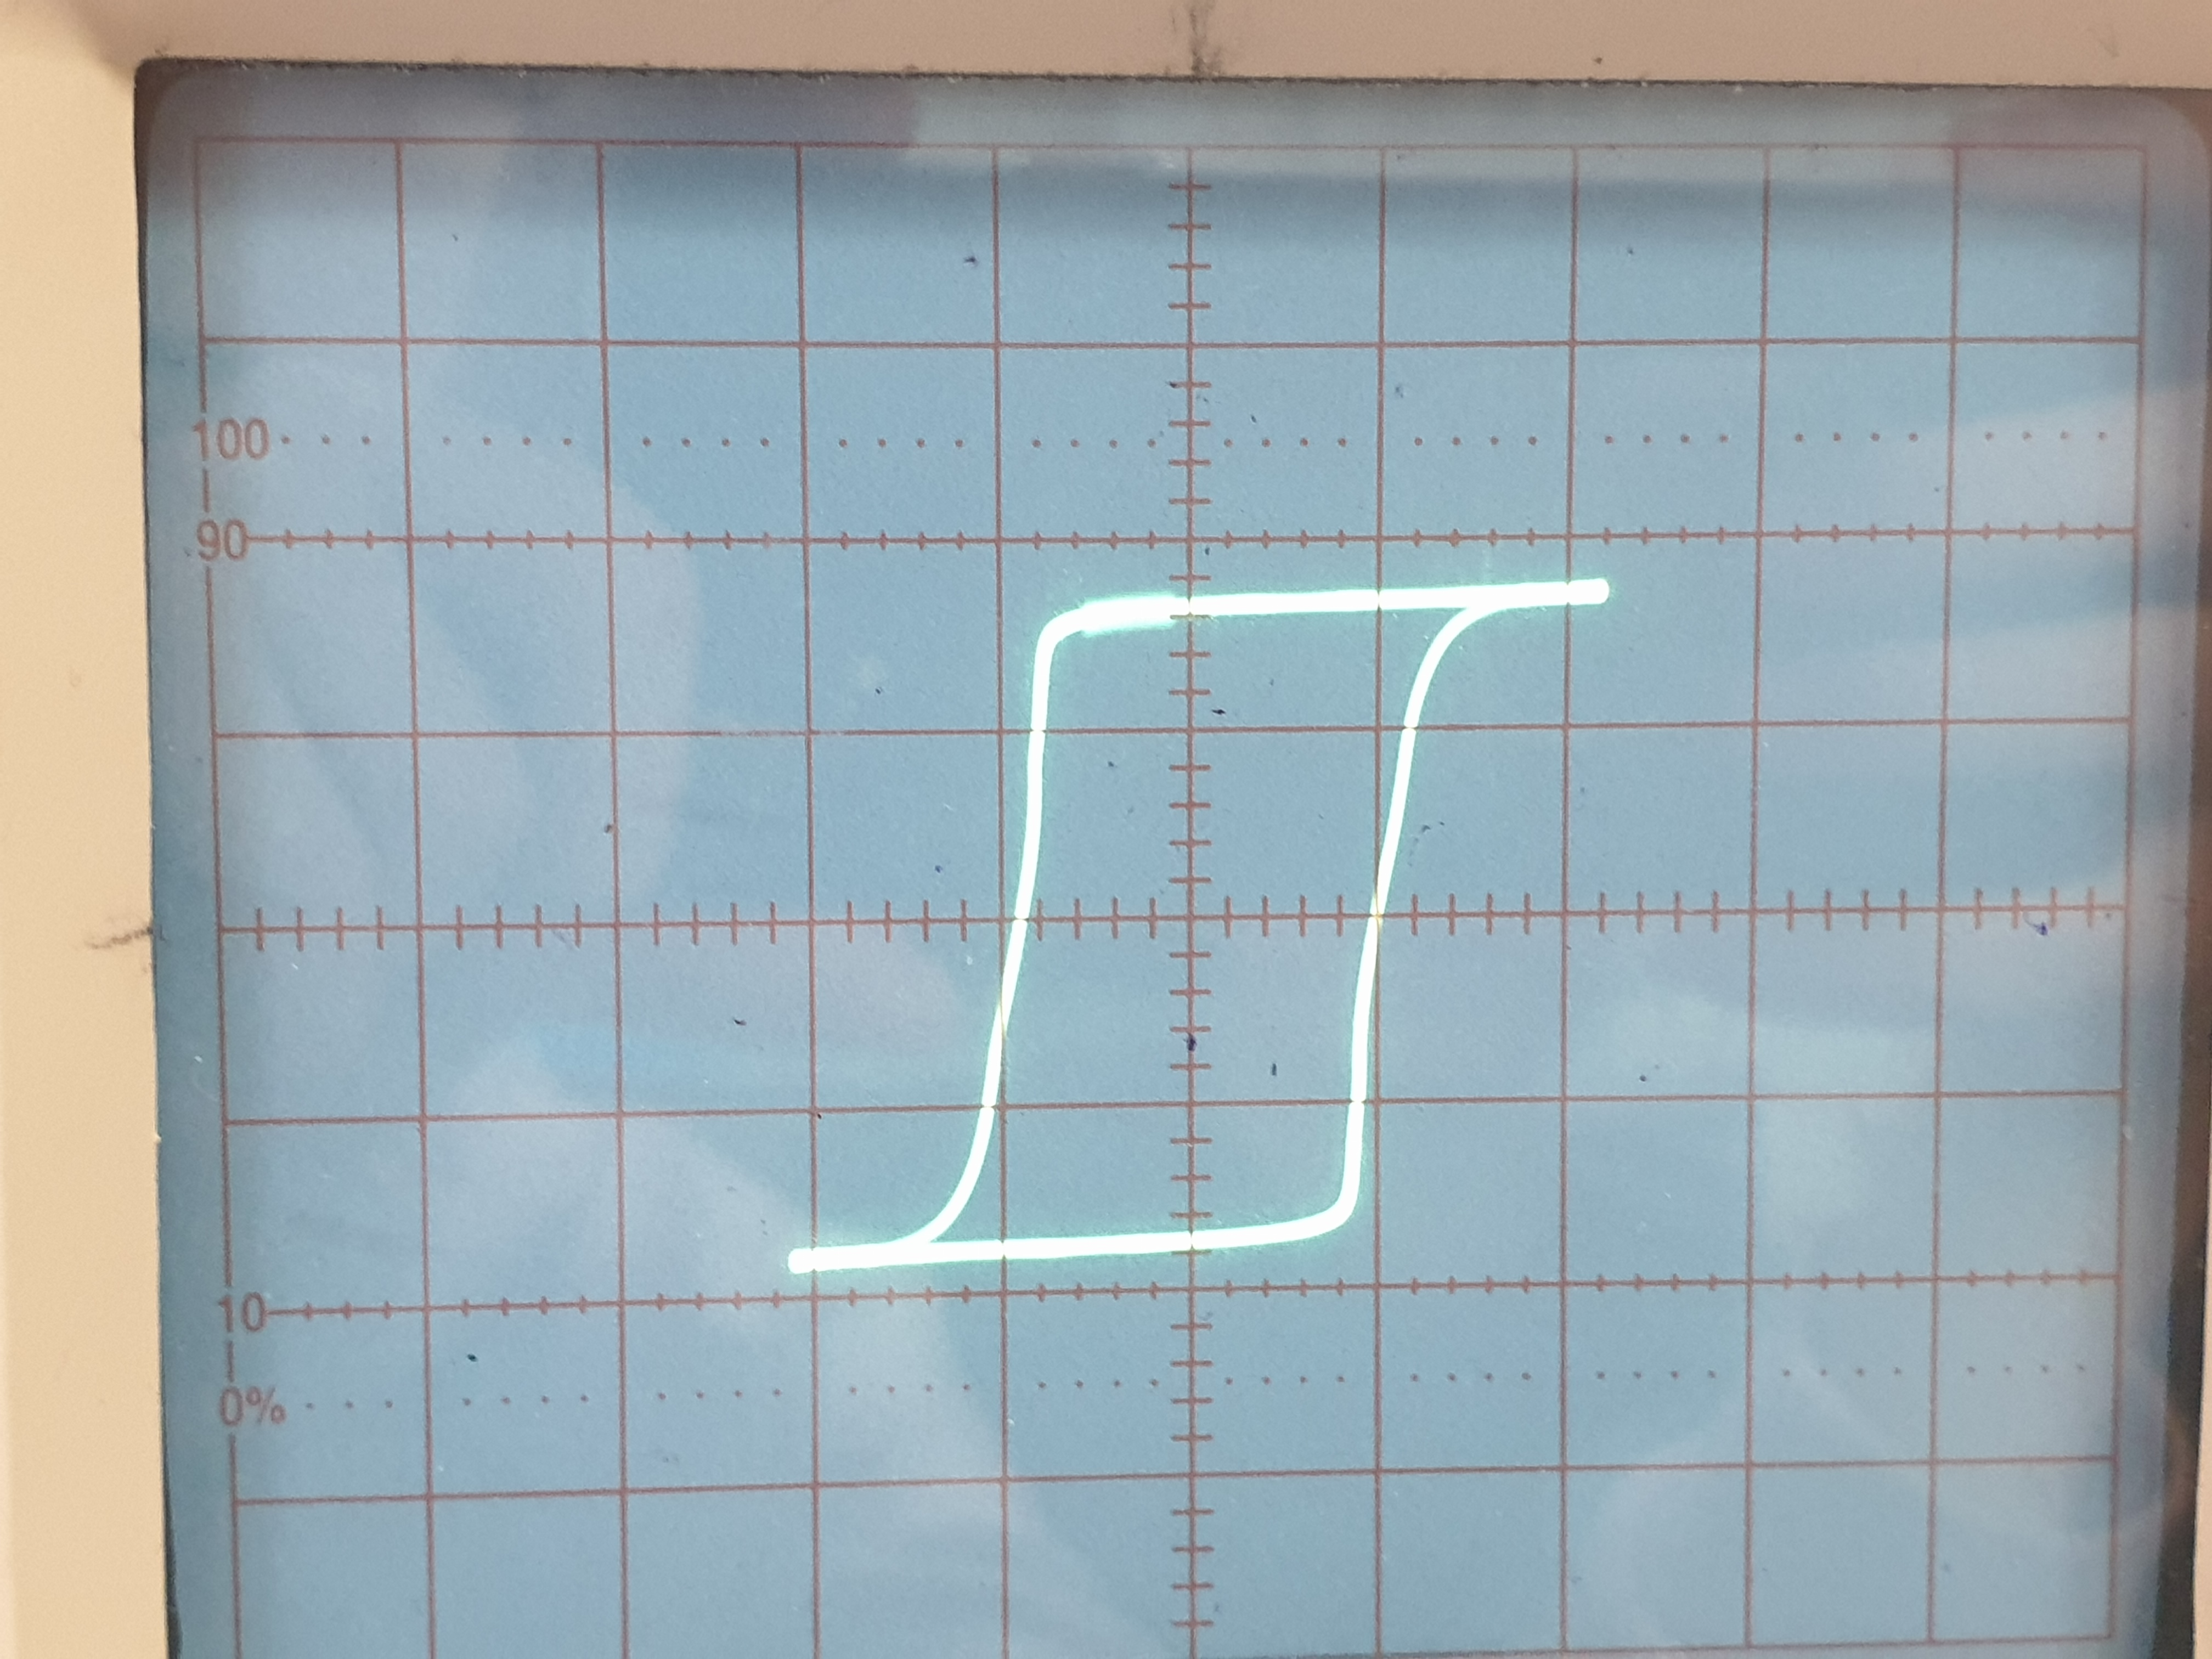
\includegraphics[width = 0.8\textwidth]{2-1.jpg}
    \caption{Петля гистерезиса для пермаллоя}
\end{figure}

Измерения будем проводить с чувствительностями:
\[ K_X = 0.048\; V/cell,\; K_Y = 0.038\; V/cell  \]

Расчитаем цену деления наряжённости поля $H$ и индукции $B$:
\[ H = \frac{IN_0}{2\pi R} = 25.5\; A/(m\cdot cell) \]
\[ B = \frac{R_uC_u}{SN_u}U_{out} = 0.77\; T/cell \]
Теперь расчитаем коэрцетивную силу $H_c$ и индукцию насыщения $B_s$ для пермаллоя:
\[ H_c = 22.9\; A/m \]
\[ B_s = 1.31\; T \]

Изменяя ток $I_{act}$ получим кривую насыщения:
\begin{figure}[H]
    \centering
    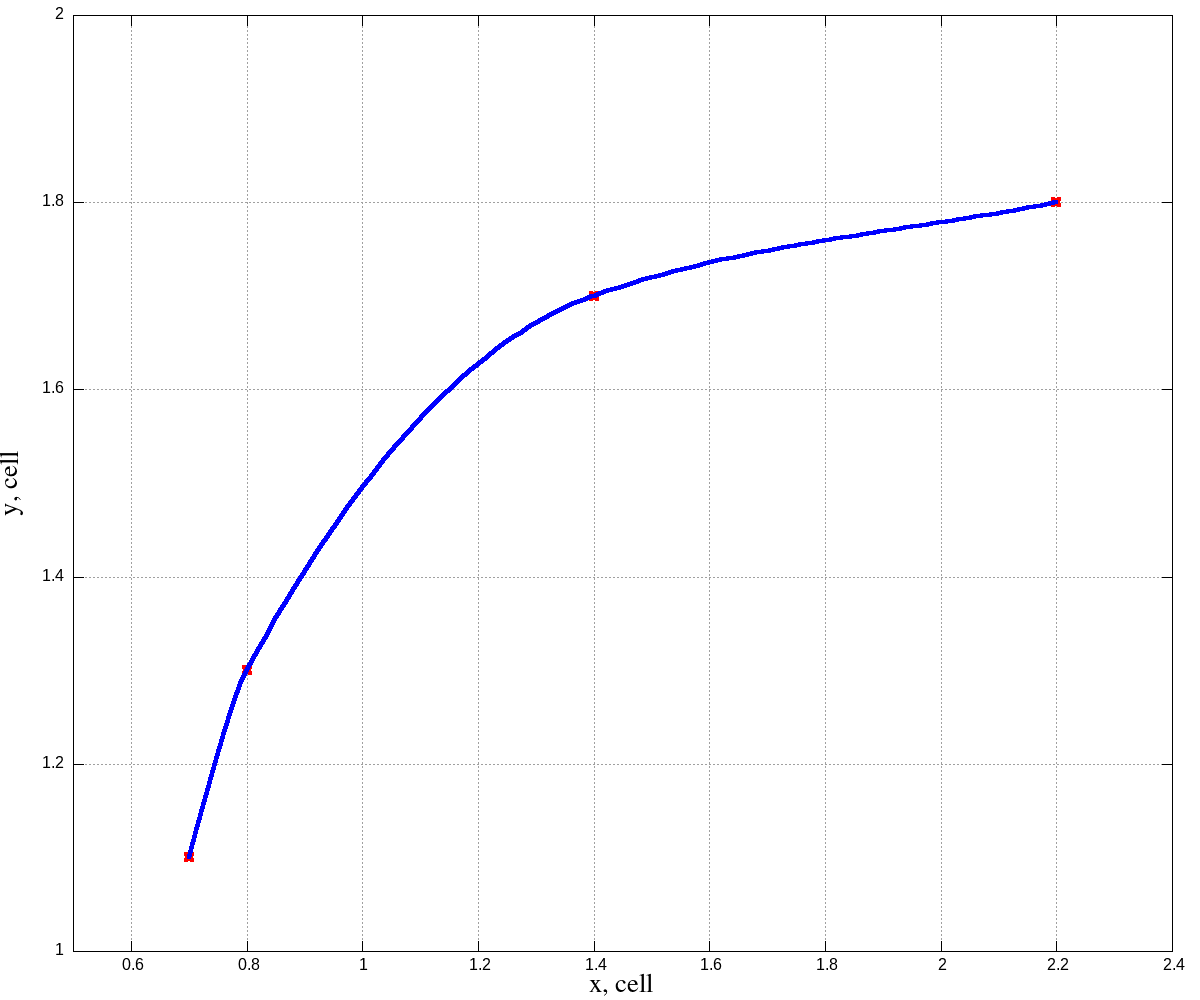
\includegraphics[width = 0.8\textwidth]{2-d.png}
    \caption{Кривая насыщения для пермаллоя}
\end{figure}

\subsubsection{Феррит}
В ходе изучения петли гисерезиса для феррита была получено изображение:
\begin{figure}[H]
    \centering
    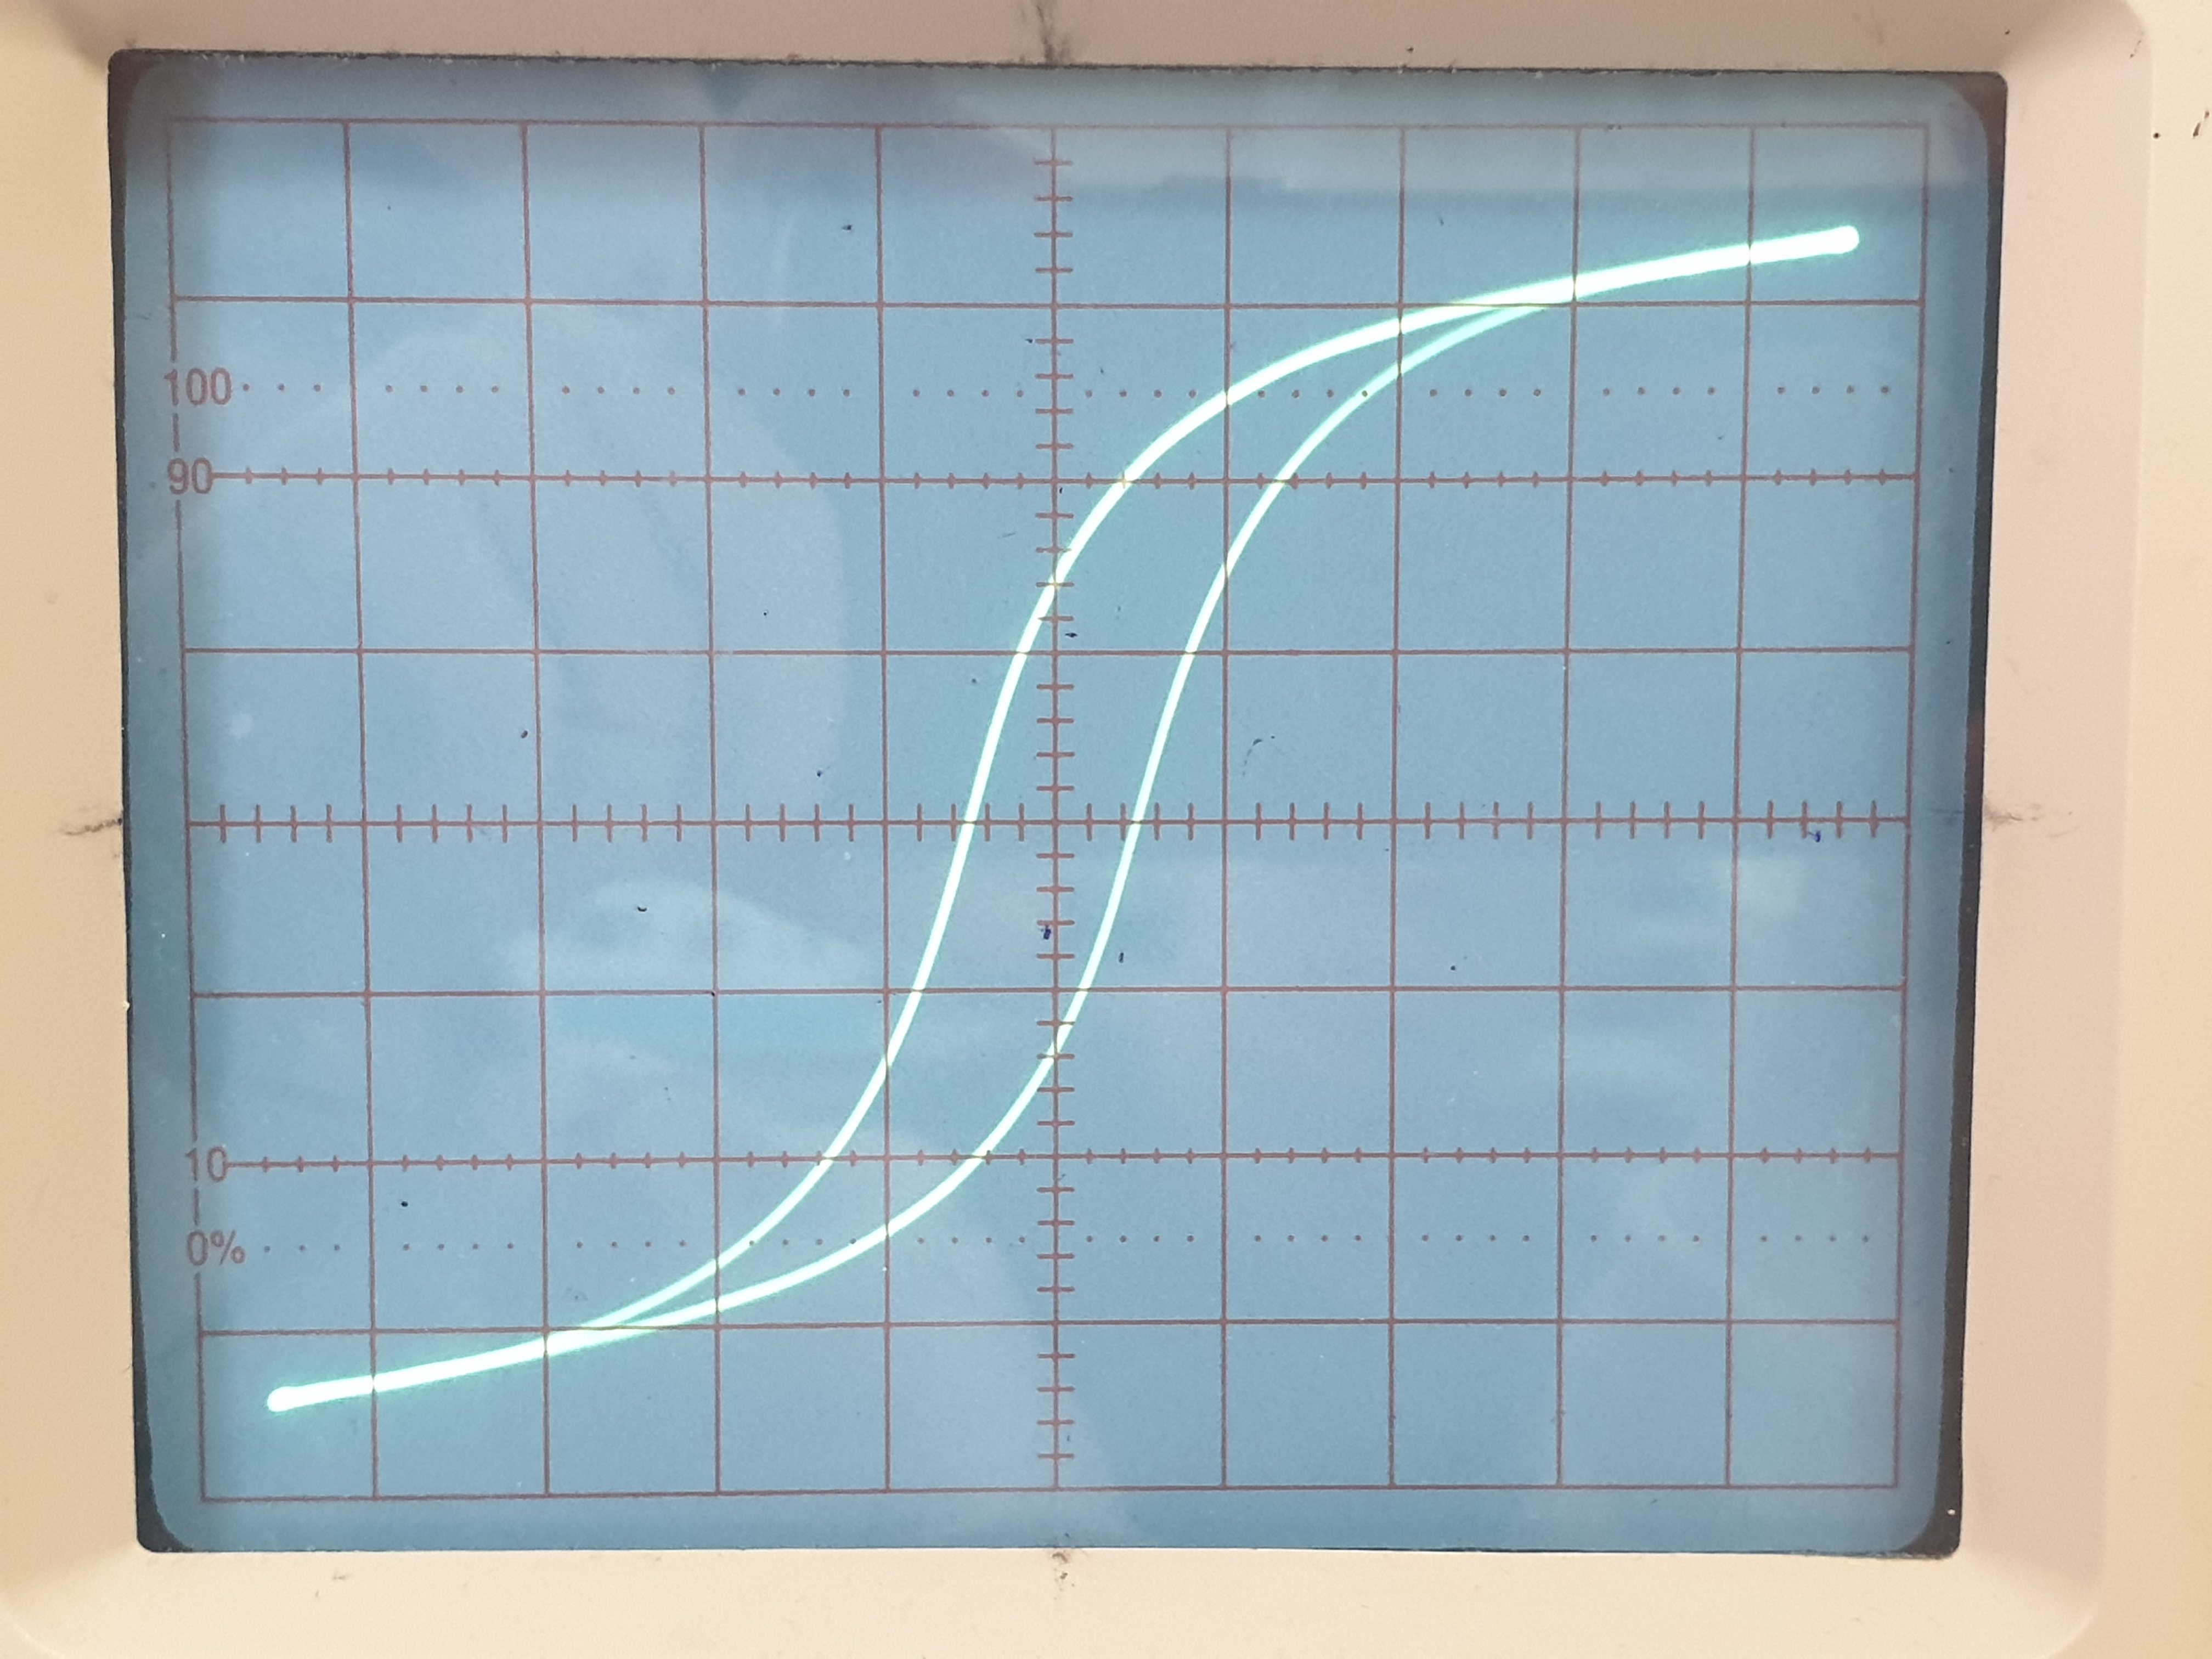
\includegraphics[width = 0.8\textwidth]{3-1.jpg}
    \caption{Петля гистерезиса для феррита}
\end{figure}

Измерения будем проводить с чувствительностями:
\[ K_X = 0.048\; V/cell,\; K_Y = 0.015\; V/cell  \]

Расчитаем цену деления наряжённости поля $H$ и индукции $B$:
\[ H = \frac{IN_0}{2\pi R} = 40.3\; A/(m\cdot cell) \]
\[ B = \frac{R_uC_u}{SN_u}U_{out} = 0.05\; T/cell \]
Теперь расчитаем коэрцетивную силу $H_c$ и индукцию насыщения $B_s$ для феррита:
\[ H_c = 20.15\; A/m \]
\[ B_s = 0.07\; T \]

Изменяя ток $I_{act}$ получим кривую насыщения:
\begin{figure}[H]
    \centering
    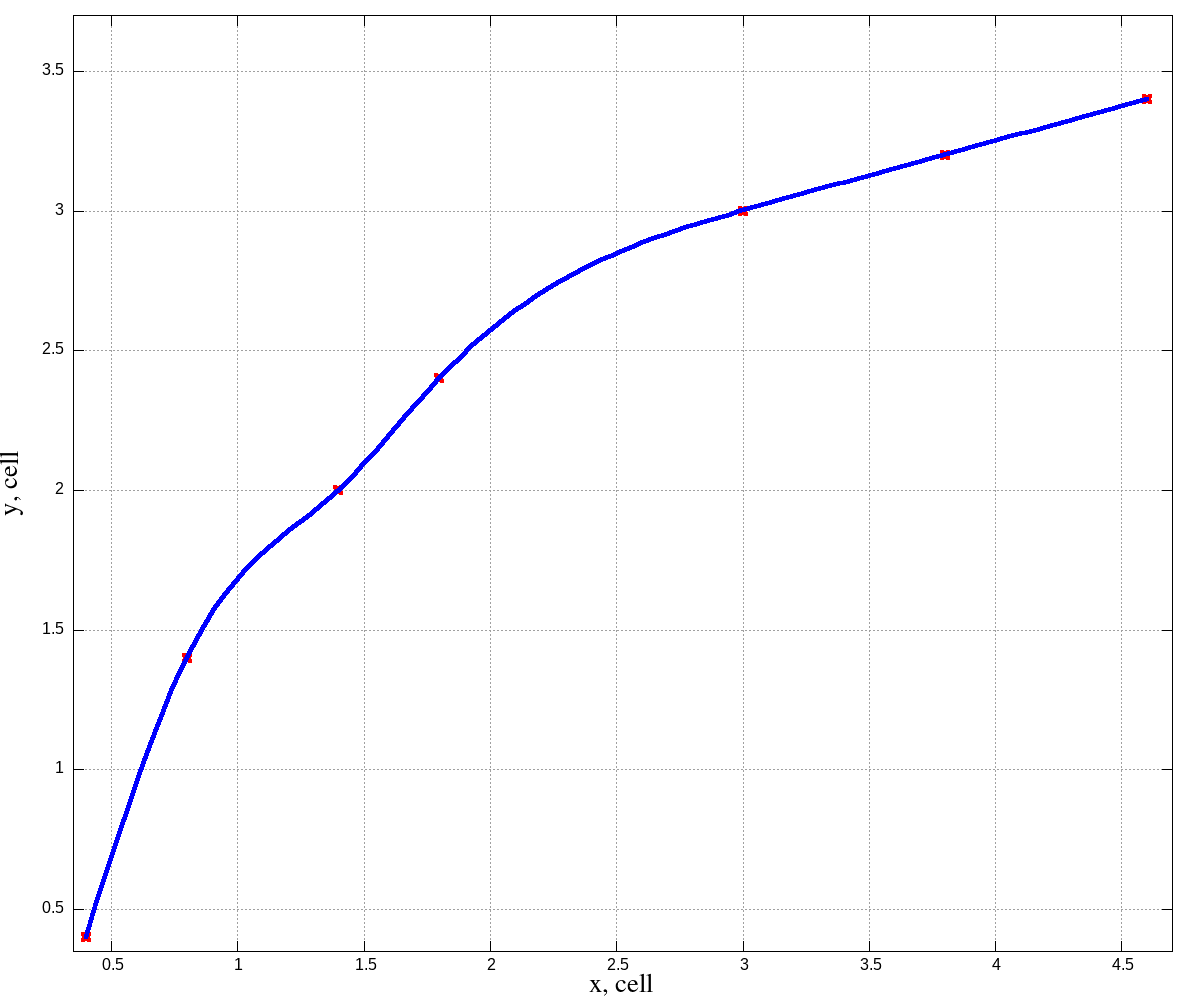
\includegraphics[width = 0.8\textwidth]{3-d.png}
    \caption{Кривая насыщения для феррита}
\end{figure}

\section{Выводы}
\begin{enumerate}
    \item В ходе проведённой работы были изучены петли гистерезиса различных феромагнитных материалов.
Были вычисленны характерные параметры (коэрцетивное поле и индукция насыщения) для каждого из образцов.
Полученные значения значительно отличатся от табличных, что может свидетельствовать об ошибках экспериментаторов
во время измерений или некорректной обрнаботки результатов.
    \item Были качественно получены кривые насыщения для каждого из образцов
\end{enumerate}
\end{document}